% ZMap User Manual
% Author: Gemma Barson
%
% Run the following command twice to create a pdf of this manual
% (two runs are necessary to make sure all of the cross-references
% are up to date):
%
%    pdflatex ZMap_User_Manual.tex
%
\documentclass[letterpaper]{article}
\usepackage[latin1]{inputenc}
\usepackage[T1]{fontenc}
\usepackage[english]{babel}
\usepackage{amsmath}
\usepackage{amssymb,amsfonts,textcomp}
\usepackage{color}
\usepackage{xcolor}
\usepackage{array}
\usepackage{supertabular}
\usepackage{hhline}
\usepackage{hyperref}
\usepackage{titlesec}
\hypersetup{colorlinks=true, linkcolor=blue, citecolor=blue, filecolor=blue, urlcolor=blue, pdftitle=ZMap User Manual, pdfauthor=Gemma Guest, pdfsubject=, pdfkeywords=}
\usepackage[pdftex]{graphicx}
% Paragraph styles
\setlength{\parindent}{0pt}
% Text styles
\newcommand\textstyleInternetlink[1]{\textcolor{blue}{#1}}
\newcommand\textstyleSourceText[1]{\texttt{#1}}
\newcommand\textstyleFootnoteSymbol[1]{\textsuperscript{#1}}
\definecolor{darkblue}{rgb}{0.2,0.3,0.5}
\definecolor{lightblue}{rgb}{0.3,0.5,0.8}
%\DeclareFixedFont{\sectionfont}{T1}{phv}{bx}{n}{16pt}
%\DeclareFixedFont{\sectionfont}{T1}{phv}{bx}{n}{14pt}
%\DeclareFixedFont{\subsectionfont}{T1}{phv}{bx}{n}{12pt}
\titleformat{\section} {\normalfont\LARGE\bf\color{darkblue}}{\thesection}{1em}{}
\titleformat{\section} {\normalfont\large\bf\color{lightblue}}{\thesection}{1em}{}
\titleformat{\subsection} {\normalfont\normalsize\bf\color{lightblue}}{\thesubsection}{1em}{}
% Outline numbering
\setcounter{secnumdepth}{0}
\makeatletter
\newcommand\arraybslash{\let\\\@arraycr}
\makeatother
% List styles
\newcommand\liststyleLi{%
\renewcommand\labelitemi{{\textbullet}}
\renewcommand\labelitemii{{\textbullet}}
\renewcommand\labelitemiii{{\textbullet}}
\renewcommand\labelitemiv{{\textbullet}}
}
\newcommand\liststyleLii{%
\renewcommand\labelitemi{{\textbullet}}
\renewcommand\labelitemii{{\textbullet}}
\renewcommand\labelitemiii{{\textbullet}}
\renewcommand\labelitemiv{{\textbullet}}
}
\newcommand\liststyleLiii{%
\renewcommand\labelitemi{{\textbullet}}
\renewcommand\labelitemii{{\textbullet}}
\renewcommand\labelitemiii{{\textbullet}}
\renewcommand\labelitemiv{{\textbullet}}
}
\newcommand\liststyleWWviiiNumxxxvi{%
\renewcommand\labelitemi{{\textbullet}}
\renewcommand\labelitemii{o}
\renewcommand\labelitemiii{[F0A7?]}
\renewcommand\labelitemiv{[F0B7?]}
}
\newcommand\liststyleLiv{%
\renewcommand\labelitemi{{\textbullet}}
\renewcommand\labelitemii{${\circ}$}
\renewcommand\labelitemiii{${\blacksquare}$}
\renewcommand\labelitemiv{{\textbullet}}
}
\newcommand\liststyleWWviiiNumxxxi{%
\renewcommand\theenumi{\arabic{enumi}}
\renewcommand\theenumii{\alph{enumii}}
\renewcommand\theenumiii{\roman{enumiii}}
\renewcommand\theenumiv{\arabic{enumiv}}
\renewcommand\labelenumi{\theenumi.}
\renewcommand\labelenumii{\theenumii.}
\renewcommand\labelenumiii{\theenumiii.}
\renewcommand\labelenumiv{\theenumiv.}
}
\newcommand\liststyleWWviiiNumxxxv{%
\renewcommand\labelitemi{{\textbullet}}
\renewcommand\labelitemii{o}
\renewcommand\labelitemiii{[F0A7?]}
\renewcommand\labelitemiv{[F0B7?]}
}
\newcommand\liststyleWWviiiNumxiii{%
\renewcommand\labelitemi{{\textbullet}}
\renewcommand\labelitemii{o}
\renewcommand\labelitemiii{[F0A7?]}
\renewcommand\labelitemiv{[F0B7?]}
}
\newcommand\liststyleWWviiiNumxxvii{%
\renewcommand\labelitemi{{\textbullet}}
\renewcommand\labelitemii{o}
\renewcommand\labelitemiii{[F0A7?]}
\renewcommand\labelitemiv{[F0B7?]}
}
\newcommand\liststyleWWviiiNumxxvi{%
\renewcommand\labelitemi{{\textbullet}}
\renewcommand\labelitemii{o}
\renewcommand\labelitemiii{[F0A7?]}
\renewcommand\labelitemiv{[F0B7?]}
}
\newcommand\liststyleWWviiiNumxvi{%
\renewcommand\labelitemi{{\textbullet}}
\renewcommand\labelitemii{o}
\renewcommand\labelitemiii{[F0A7?]}
\renewcommand\labelitemiv{[F0B7?]}
}
\newcommand\liststyleWWviiiNumxxxvii{%
\renewcommand\labelitemi{{\textbullet}}
\renewcommand\labelitemii{o}
\renewcommand\labelitemiii{[F0A7?]}
\renewcommand\labelitemiv{[F0B7?]}
}
\newcommand\liststyleWWviiiNumxx{%
\renewcommand\labelitemi{{\textbullet}}
\renewcommand\labelitemii{o}
\renewcommand\labelitemiii{[F0A7?]}
\renewcommand\labelitemiv{[F0B7?]}
}
% Page layout (geometry)
\setlength\voffset{-1in}
\setlength\hoffset{-1in}
\setlength\topmargin{2.54cm}
\setlength\oddsidemargin{3.175cm}
\setlength\textheight{21.363003cm}
\setlength\textwidth{15.240001cm}
\setlength\footskip{1.497cm}
\setlength\headheight{0cm}
\setlength\headsep{0cm}
% Footnote rule
\setlength{\skip\footins}{0.119cm}
\renewcommand\footnoterule{\vspace*{-0.018cm}\setlength\leftskip{0pt}\setlength\rightskip{0pt plus 1fil}\noindent\textcolor{black}{\rule{0.25\columnwidth}{0.018cm}}\vspace*{0.101cm}}
% Pages styles
\makeatletter
\newcommand\ps@Standard{
  \renewcommand\@oddhead{}
  \renewcommand\@evenhead{}
  \renewcommand\@oddfoot{\thepage{}}
  \renewcommand\@evenfoot{\@oddfoot}
  \renewcommand\thepage{\arabic{page}}
}
\newcommand\ps@FirstPage{
  \renewcommand\@oddhead{}
  \renewcommand\@evenhead{}
  \renewcommand\@oddfoot{}
  \renewcommand\@evenfoot{}
  \renewcommand\thepage{\arabic{page}}
}
\makeatother
\pagestyle{Standard}
\setlength\tabcolsep{1mm}
\renewcommand\arraystretch{1.3}
% footnotes configuration
\makeatletter
\renewcommand\thefootnote{\arabic{footnote}}
\makeatother
\newcounter{Figure}
\renewcommand\theFigure{\arabic{Figure}}

\definecolor{darkgreen}{RGB}{0,150,0}


\title{ZMap User Manual}
\author{Gemma Barson}
\date{2011-01-18}

\begin{document}

\setcounter{page}{1}\pagestyle{Standard}


\thispagestyle{FirstPage}
{\centering\sffamily\bfseries\color[rgb]{0.0,0.27058825,0.5254902}
\Huge\bf{ZMap User Manual}\par}

\bigskip

{\centering\large{Written by and contributions from:}\par
\large{Gemma Guest} {\textless}\href{mailto:gb10@sanger.ac.uk}{gb10@sanger.ac.uk}{\textgreater}\par
\large{Charlie Stewart}\par
\large{Laurens Wilming}\par
\large{Ed Griffiths}\par
\large{James Gilbert}\par
\large{Jennifer Harrow}\par
}


\bigskip

{\centering\large{Wellcome Trust Sanger Institute}\par}
{\centering16 March 2015\par}



\clearpage
{\color[rgb]{0.0,0.27058825,0.5254902}\section[Revision History]{Revision History}}
\hypertarget{RefHeading334316266717}{}

\begin{center}
\tablehead{}
\begin{supertabular}{|m{8cm}|m{3.2849998cm}|m{3.282cm}|}
\hline
\bfseries Revision &
\bfseries Date &
\bfseries Author\\\hline
 First revision (ZMap v1.5.0) &
 16/03/2015 &
 Gemma Guest\\\hline
 Updated for ZMap v2.5.1 &
 12/02/2016 &
 Gemma Guest\\\hline
 &
 &
 \\\hline
 &
 &
 \\\hline
 &
 &
 \\\hline
 &
 &
 \\\hline
 &
 &
 \\\hline
 &
 &
 \\\hline
\end{supertabular}
\end{center}

\bigskip

\setcounter{tocdepth}{10}
\renewcommand\contentsname{Contents}

\clearpage\tableofcontents

\clearpage
\section{Introduction}

ZMap is a software package that provides a visualisation and editing tool for genomic features. The software is written in C/C++, utilising the gnome toolkit (GTK2) to draw features on a canvas. ZMap accepts input from multiple sources in multiple formats across multiple genomes and is written in a way so that the addition of further formats is made as trivial as possible. Currently the list of formats includes GFF and DAS, which may reside in any one of; a file, an acedb instance, an http server. Multiple genomes and their associated features can be displayed in a single view as aligned blocks providing support for comparative annotation. ZMap privides facilities for editing and creating features, which can then be saved to a GFF file.

ZMap is part of the Otter annotation suite and contains a protocol for two-way communication with Otter so that it operates seamlessly as an additional display within Otter.

ZMap can call tools from the SeqTools suite of sequence visualisation tools to analyse alignments in more detail.

\section{Starting ZMap}
There are several ways to run ZMap depending on the data sources you want to use.

\subsection{Running ZMap on a GFF file}
To run ZMap standalone on one or more GFF files, simply pass the file name(s) on the command line:
\begin{verbatim}
zmap file1.gff file2.gff
\end{verbatim}

The sequence region will default to the region available in the GFF file. Alternatively, you can specify the sequence/region by passing the \texttt{--sequence}, \texttt{--start} and \texttt{--end} arguments on the command-line.

If all of the files contain the same reference sequence, then their contents will be shown in the same view. If the files contain multiple sequences/regions, then they will be shown in multiple views.

\subsection{Choosing sources on startup}
If you run ZMap without any arguments then you will be presented with the Main Window where you can choose data sources to load (see Figure \ref{img_main_window}).

\begin{figure}
\centering
\color[rgb]{0.30980393,0.5058824,0.7411765}
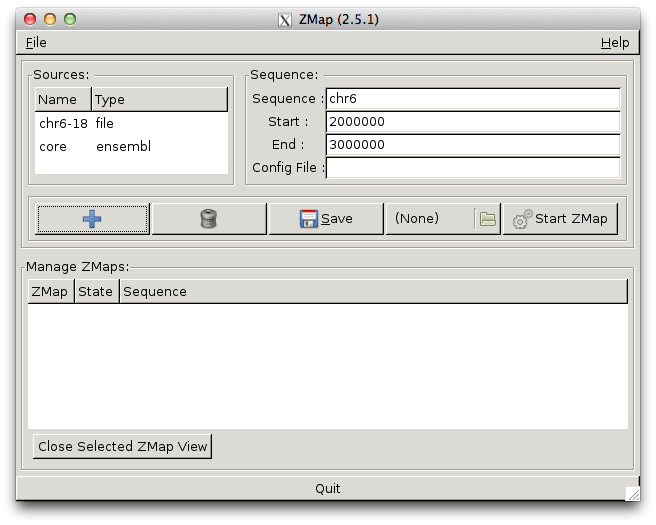
\includegraphics[width=15.231cm]{img_main_window.png}
\caption{ZMap's Main Window. Use the '+' button to add new sources, enter the sequence details for the region you want to view, and then click 'Start ZMap'.}
\label{img_main_window}
\end{figure}

Click on the '+' button to add a new source. This will open the Create Source dialog. From the drop-down menu, select the type of source. Choose 'File' for a local/remote file (figure \ref{img_create_source_file}) or 'Ensembl' for an Ensembl database (figure \ref{img_create_source_ensembl}).

For File sources, you just need to enter the path of the file (or URL if it is a remote file). You also need to enter a name for the source - this can be anything you like.

For Ensembl sources, the public host details are pre-filled for you by default. You may change these if you wish but the public host should be fine for most users (note that a password is not required). You can click the magnifying glass icon next to the 'Database' box to search for available databases in the host (figure \ref{img_create_source_ensembl_search_db}). You may optionally also enter a list of featuresets or biotypes that you are interested in - in this case, ZMap will only load features of those types; otherwise, ZMap will load all of the features from the database. You can click the magnifying glass icon next to the featuresets/biotypes boxes to search for available featuresets/biotypes. Note that you can select multiple featuresets/biotypes from the search box by holding down Ctrl (for individual selection) or Shift (for range selection) when you click with the mouse button. You can also enter multiple featuresets/biotypes directly into the Create Source dialog as a semi-colon separated list.

\begin{figure}
\centering
\color[rgb]{0.30980393,0.5058824,0.7411765}
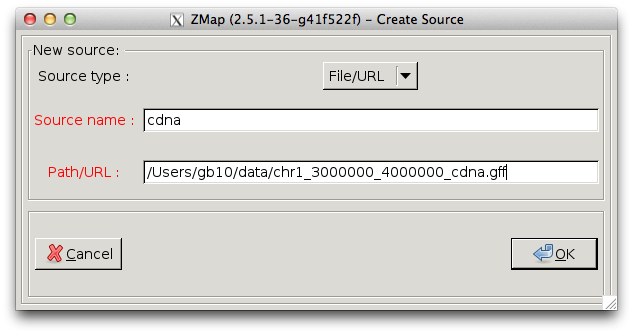
\includegraphics[width=15.231cm]{img_create_source_file.png}
\caption{Create a new file source}
\label{img_create_source_file}
\end{figure}

\begin{figure}
\centering
\color[rgb]{0.30980393,0.5058824,0.7411765}
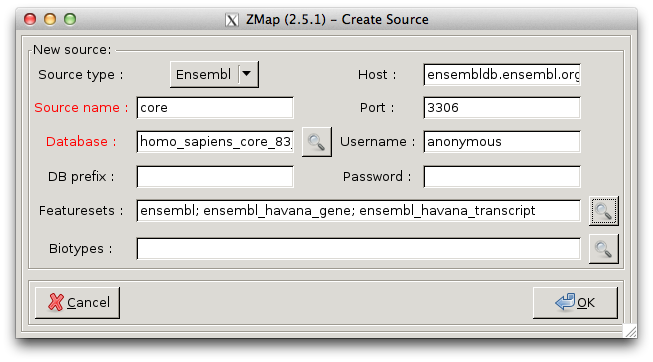
\includegraphics[width=15.231cm]{img_create_source_ensembl.png}
\caption{Create a new Ensembl source. Click on the magnifying glass icons to search for databases/featuresets/biotypes to load.}
\label{img_create_source_ensembl}
\end{figure}

\begin{figure}
\centering
\color[rgb]{0.30980393,0.5058824,0.7411765}
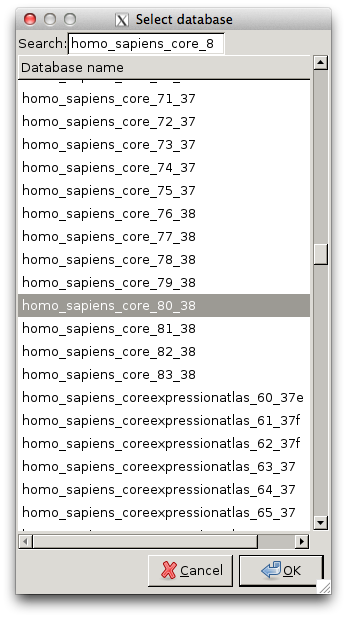
\includegraphics[width=8cm]{img_create_source_ensembl_search_db.png}
\caption{Search a list of available Ensembl databases. Type text in the Search box to jump to items containing that text. You can use the up/down arrows to jump to the next/previous item with the same text.}
\label{img_create_source_ensembl_search_db}
\end{figure}

After you click OK on the Create Source dialog, the new source will appear in the Main Window. You can enter multiple sources in the same way. If you want to remove a source, select it in the list and click the delete button. You also need to enter the sequence details for the region you want to load. Then click 'Start ZMap' to open ZMap on that region. You can edit the sources/sequence details at any time and click 'Start ZMap' again to start a new ZMap on a different region.

You can save the source details to a config file so that they can easily be re-loaded later. Simply click the Save button and select a file location. To re-use the config, you can either open the Main Window again and select the file using the file chooser button, or you can run ZMap on the file from the command-line as follows:
\begin{verbatim}
zmap --conf_file=/path/to/file
\end{verbatim}

\subsection{Running ZMap with a config file}
If you have several sources, it can be convenient to specify them in a config file rather than typing them on the command-line. You can also then set up many different options and styles to use for these sources. To use a local GFF file as a source, a simple config file would look something like this:
\begin{verbatim}
[ZMap]
# The list of sources
sources=chr6-18

# Sequence name/start/end can be specified here, on the command-line, or
# omitted if they are to be taken from the file
sequence=chr6-18
start=2696324
end=2864370

# Source stanzas (one per source)
[chr6-18]
url=file:////Users/gb10/work/checkout/zmap/examples/features.gff
\end{verbatim}

ZMap can then be started by passing the config file on the command line:
\begin{verbatim}
zmap --conf_file=/path/to/file
\end{verbatim}

Alternatively, the config file can be saved as \texttt{~/.ZMap/ZMap} and will be picked up by default.

\subsection{Operation within Otter}
ZMap is opened via the Tools menu bar in Otter (figure \ref{img_open_from_otterlace}).

\begin{figure}
\centering
\color[rgb]{0.30980393,0.5058824,0.7411765}
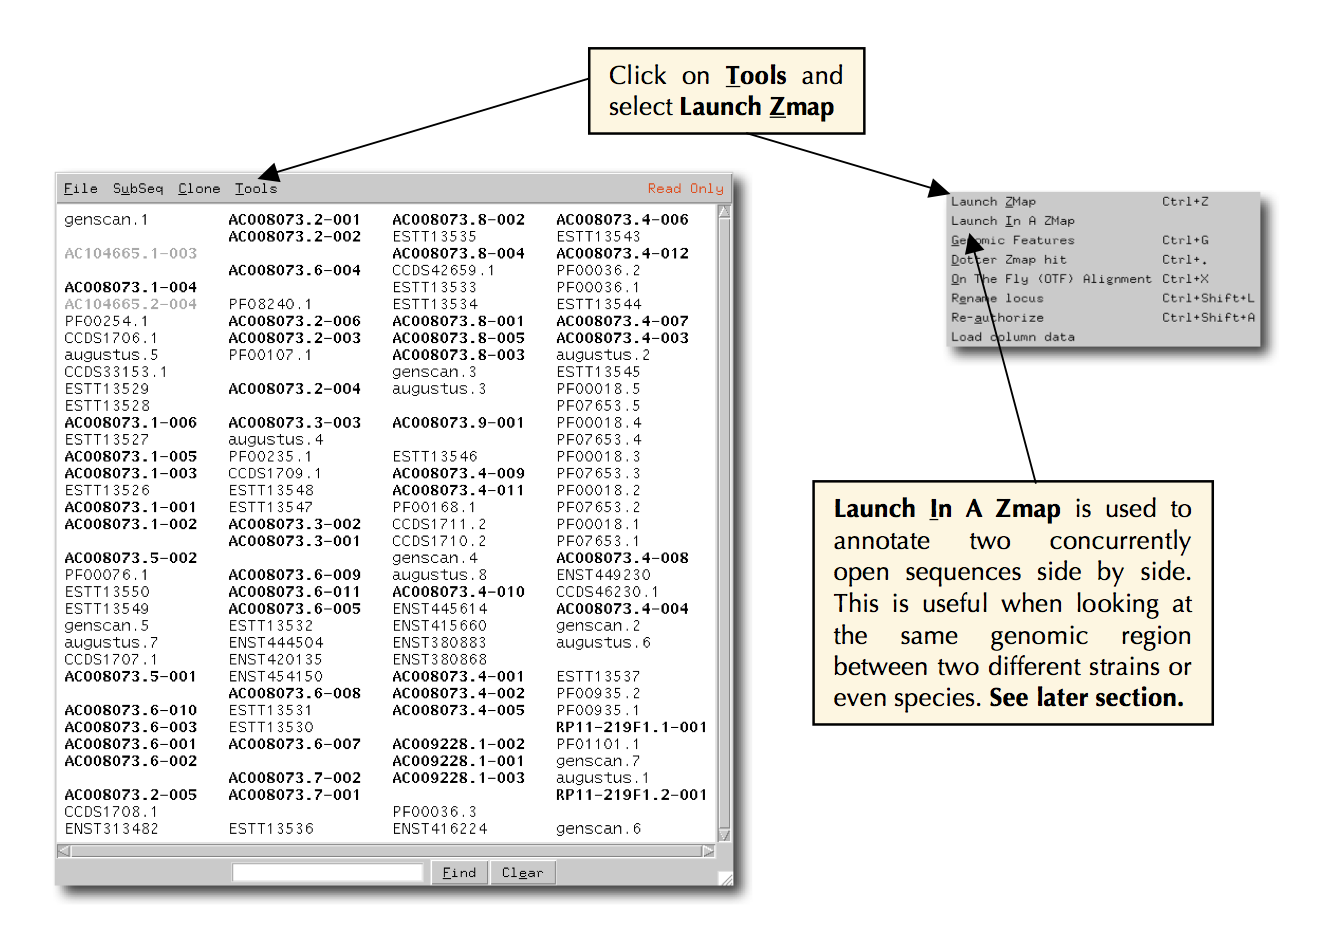
\includegraphics[width=15.231cm]{img_open_from_otterlace.png}
\caption{Opening ZMap from Otter}
\label{img_open_from_otterlace}
\end{figure}

\section{The ZMap display}

The main ZMap display (figure \ref{img_main_interface} consists of a canvas showing any analysis and annotation that is present in your region of interest, with a toolbar, information bar and menu at the top and a ruler showing the coordinates at the current position based on the current coordinate system.

\begin{figure}
\centering
\color[rgb]{0.30980393,0.5058824,0.7411765}
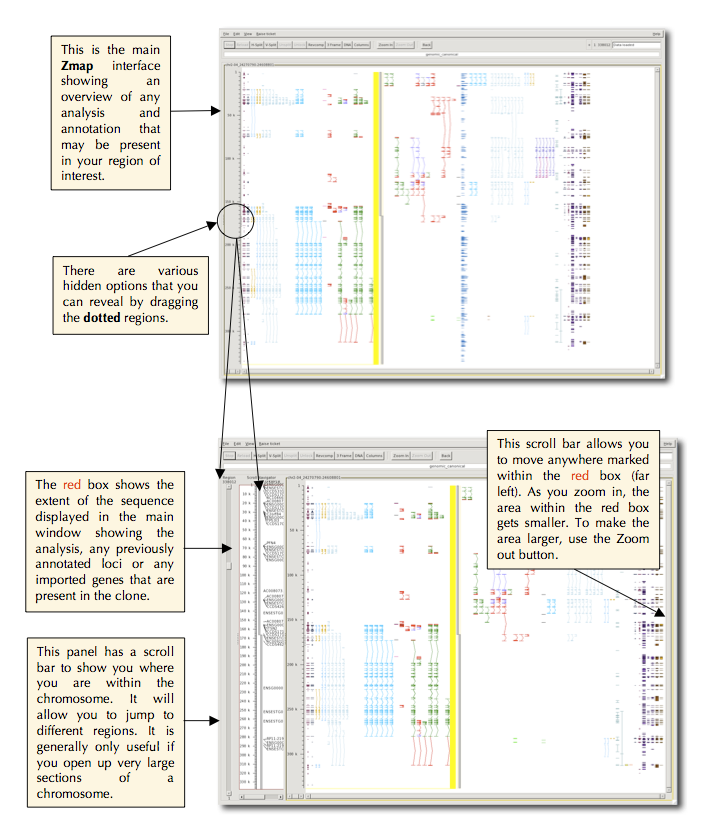
\includegraphics[width=15.231cm]{img_main_interface.png}
\caption{The main ZMap interface}
\label{img_main_interface}
\end{figure}

\subsection{Navigating}
Navigate by using the scroll bars or the middle mouse button (figure \ref{img_navigating}. By clicking the middle mouse anywhere in ZMap you will see a horizontal line. You can move this up and down and the relative position in bp will be displayed along the line.

When the button is released, the window will refresh, centering on the position of the line. You can also click in the window to make it active and use the scroll wheel to navigate up and down or achieve the same result using the scroll bar on the right hand side of the window.

If you release the mouse outside the ZMap window, you can then check the sequence position displayed, without re-centering.

\begin{figure}
\centering
\color[rgb]{0.30980393,0.5058824,0.7411765}
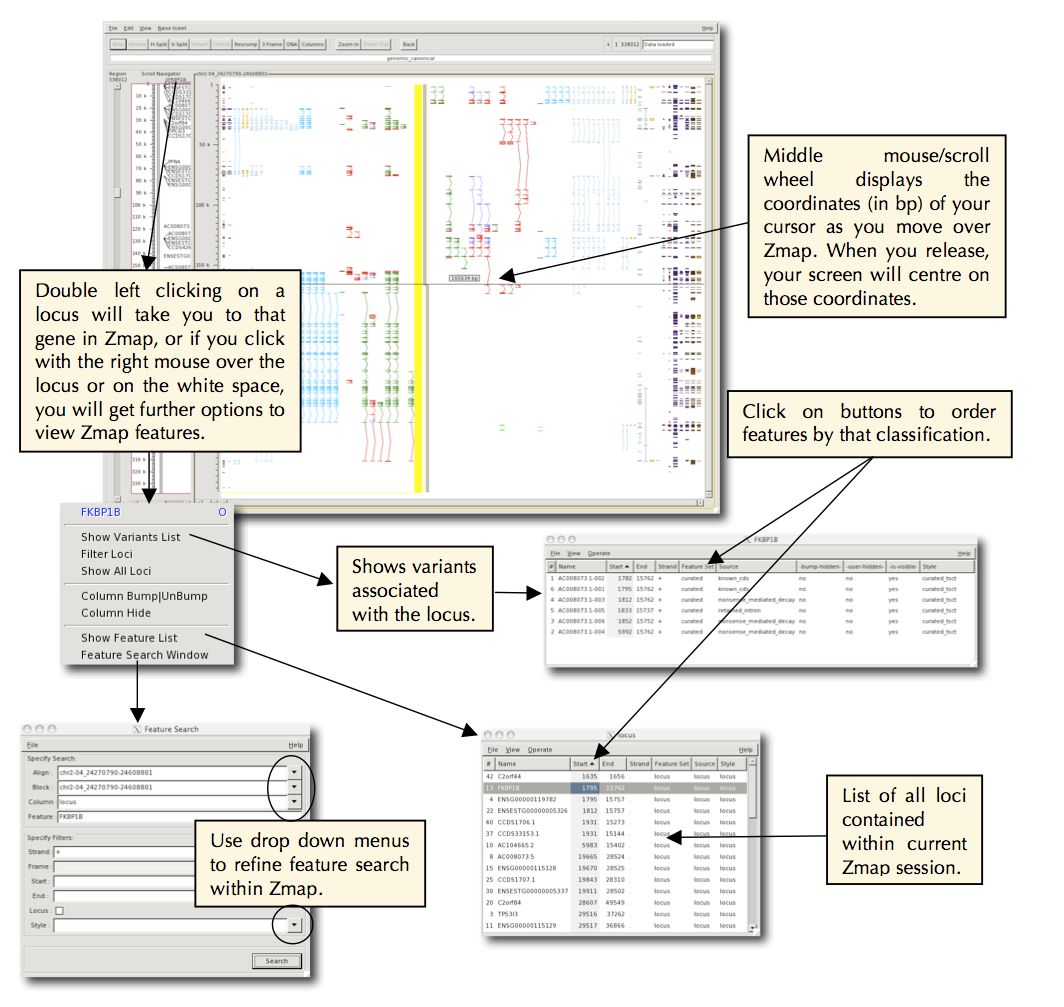
\includegraphics[width=15.231cm]{img_navigating.png}
\caption{Navigating}
\label{img_navigating}
\end{figure}

\subsection{Zooming}
See figure \ref{img_zooming}.

\begin{itemize}
\item Zoom in by using the Zoom in/Zoom out buttons on the toolbar
\item Draw with the left mouse button to lasso an area to zoom in to
\item Press the ``z'' key on the keyboard to zoom to the current focus feature.
\item Use the ``Z'' key to zoom to a whole transcript if you have one or more exons highlighted, or all HSPs if you have one HSP highlighted (HSPs are the "blocks" that you see in the homology columns, such as ESTs and protein hits). 
\end{itemize}

\begin{figure}
\centering
\color[rgb]{0.30980393,0.5058824,0.7411765}
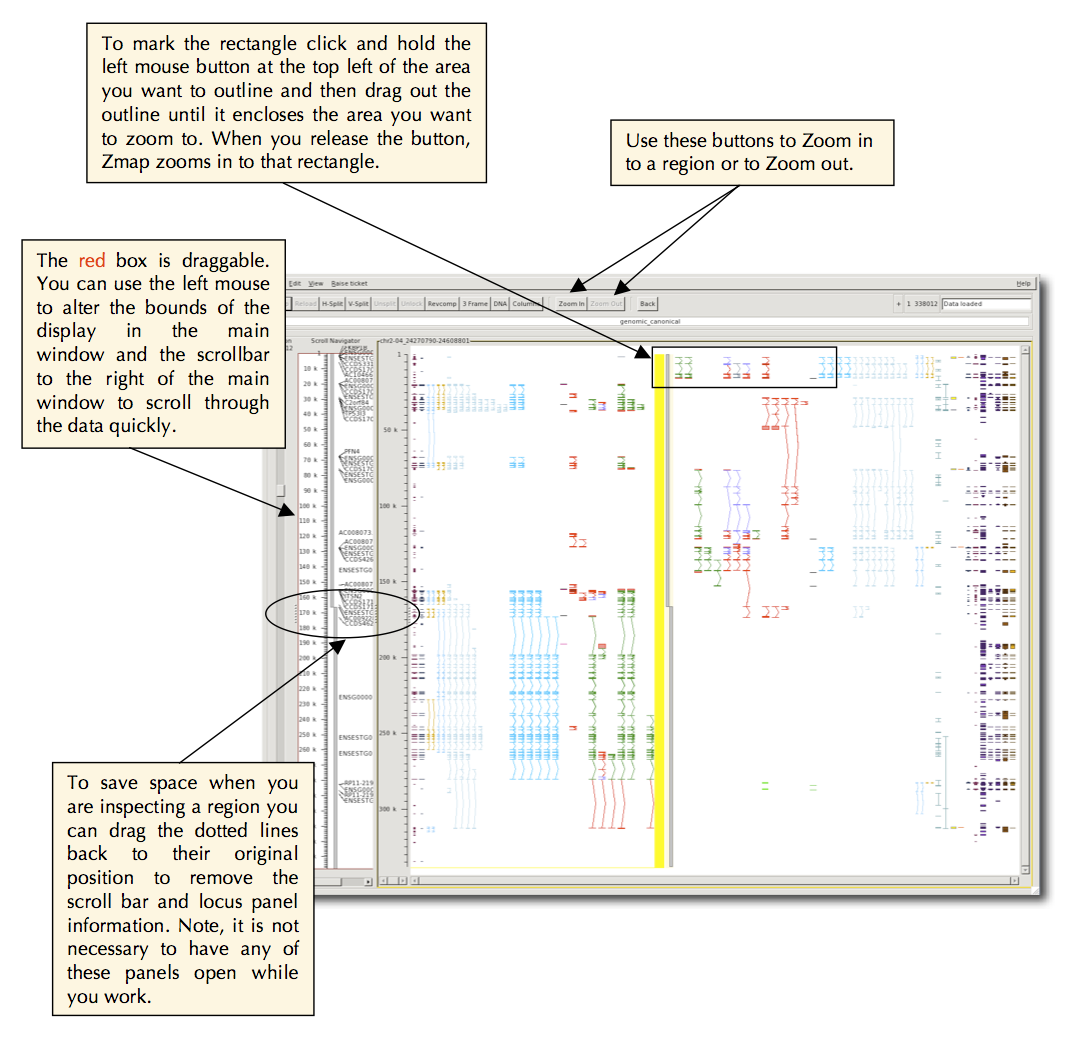
\includegraphics[width=15.231cm]{img_zooming.png}
\caption{Zooming}
\label{img_zooming}
\end{figure}

\subsection{The Focus Feature}
If you click on a column background then that column becomes the "focus" column and you can do various short cut operations on it such as pressing "b" to bump it. If you click on a feature then that feature becomes the "focus" feature and similarly you can do various short cut operations on it such as zooming in to it. (Note when you select a feature then its column automatically becomes the focus column.)

While the focus facility is useful, the focus changes every time you click on a new feature. Sometimes you want to select a "working" feature or area more permanently. To do this you can "mark" a feature or region and it will stay marked until you unmark it (see section \ref{section_marking_a_region}).

\subsection{Marking a region}
\label{section_marking_a_region}
The "marked" area remains clear, while the unmarked area above and below is shaded out with a blue hashed overlay (see figure \ref{img_focus_and_mark}). Working on a marked region is recommended when you have a large amount of data loaded, because operations are faster and the display is less cluttered.

\begin{figure}
\centering
\color[rgb]{0.30980393,0.5058824,0.7411765}
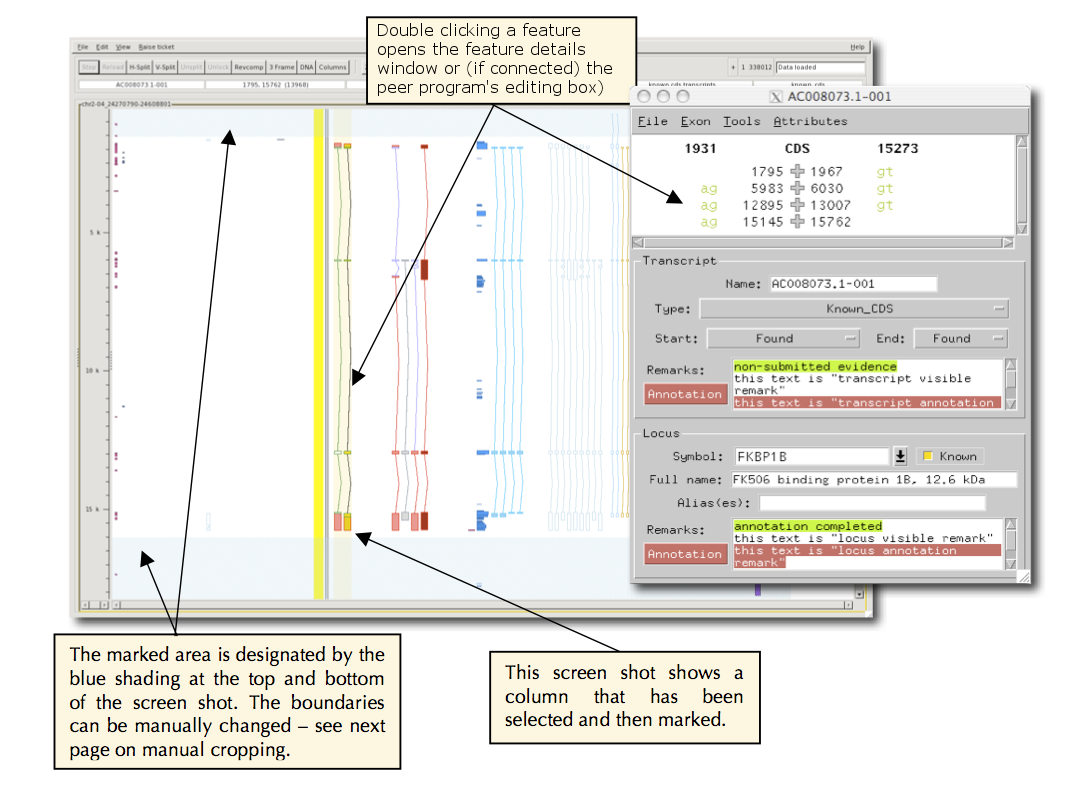
\includegraphics[width=15.231cm]{img_focus_and_mark.png}
\caption{Focus and Mark}
\label{img_focus_and_mark}
\end{figure}

\subsubsection{Mark a feature}
\begin{enumerate}
\item Select a feature to make it the focus feature.
\item Press ``m'' to mark the feature, the feature will be highlighted with a blue overlay.
\end{enumerate}

Feature marking behaves differently according to the type of feature you highlighted prior to marking and according to whether you press ``m'' or ``M'' to do the marking:

\begin{enumerate}
\item  If you press ``m'', the mark is made around all features you have highlighted, e.g. a whole transcript, a single exon, several HSPs.
\item  If you press ``M'' to do the marking around transcripts the whole transcript becomes the marked feature and the marked area extends from the start to the end of the transcript.
\item  If you press ``M'' to do the marking around alignments all the HSPs for that alignment become the marked feature and the marked area extends from the start to the end of all the HSPs.
\item  If you press ``M'' to do the marking around all other features: the feature becomes the marked feature and the marked area extends from the start to the end of the feature.
\item  If no feature is selected but an area was selected using the left button rubberband then that area is marked.
\item  If no feature or area is selected then the visible screen area minus a small top/bottom margin is marked.
\end{enumerate}

\subsubsection{Mark an area}
\begin{enumerate}
\item Select an area by holding down the left mouse button and dragging out a box to focus on that area.
\item Press "m" to mark the area.
\end{enumerate}

\subsubsection{Manual cropping of the marked borders}
You can manually change the borders of the marked area by putting your cursor over this area and using the cropping tool by clicking and holding with the left mouse button and dragging to make the area bigger or smaller.

\subsubsection{Unmark a feature}
Press "m" or "M" again, i.e. the mark key toggles marking on and off.

\subsection{General ZMap display features}
ZMap has rich feature display capabilities, which are highly configurable. Different features are displayed in distinct columns, and can be configured with many different styles as shown in figure \ref{img_features}. 

\begin{figure}
\centering
\color[rgb]{0.30980393,0.5058824,0.7411765}
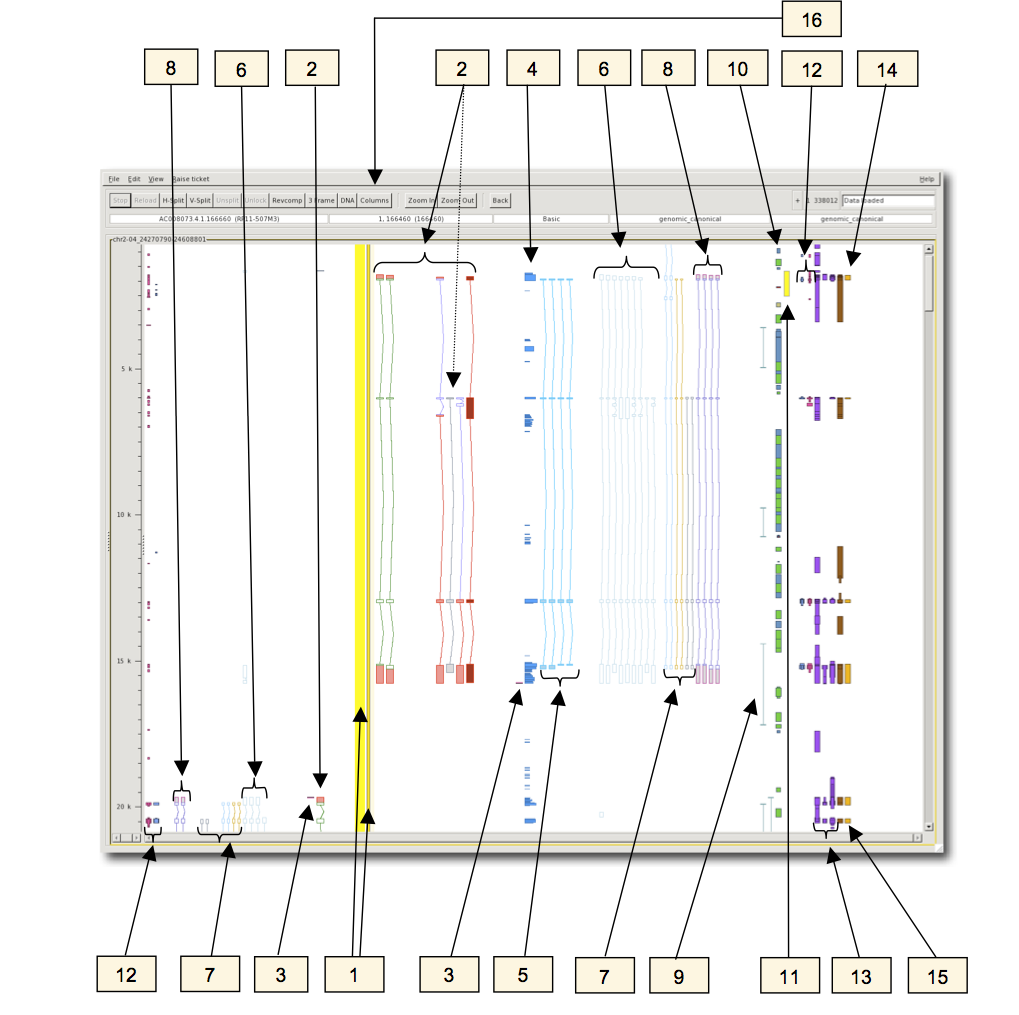
\includegraphics[width=15.231cm]{img_features.png}
\caption{Features}
\label{img_features}
\end{figure}

\begin{enumerate}
\item  The thick yellow line represents the genomic sequence; everything to the left represents the negative strand and everything to the right the positive strand. DNA matches (i.e. ESTs, mRNAs and RefSeq) and repeats have been configured so that they are all displayed to the right of the center, although they may align to either strand. Other features are configured to display in their relevant strand. The thin bar to the right is the clone that the genomic sequence is made up from. When connected to the Otter peer, double-clicking on this gives access to the DE editing window.
\item  Annotated transcripts; green is coding (CDS), red is non-coding (UTR and transcript variants) and purple shows the "coding'' region of NMD variants. Grey transcripts (see dotted line) contain exons outside the sequence slice being viewed and should not be confused with Halfwise hits.
\item  Curated features, such as PolyA features are seen as horizontal black lines.
\item  Phastcons44 - conserved regions detected using multiple sequence alignments of 44 organisms.
\item  Imported annotation from CCDS (human and mouse only).
\item  Imported transcripts via DAS source. Here PASA\_ESTs are shown.
\item  Predicted transcripts such as Genscan (pale blue), Augustus (gold) and Halfwise predictions of Pfam (grey).
\item  Imported annotation from Ensembl.
\item  gis\_pet\_ditags and chip\_pet\_ditags are indicators of transcript boundaries.
\item Repeats ( blue=Line , light green=Sine , gold=other ), tandem repeats are red.
\item CpG islands appear as yellow boxes.
\item Protein matches are strand specific - SwissProt are light blue and Trembl pink.
\item EST matches are displayed as purple blocks and are broken down into human ESTs, mouse ESTs, and other ESTs from other organisms. 5' reads are on the left and 3' on the right.
\item mRNA matches contains all species and are displayed as brown blocks,
\item RefSeq matches are the orange blocks.
\item Features and analysis available (see figure \ref{img_columns}).
\end{enumerate}

\begin{figure}
\centering
\color[rgb]{0.30980393,0.5058824,0.7411765}
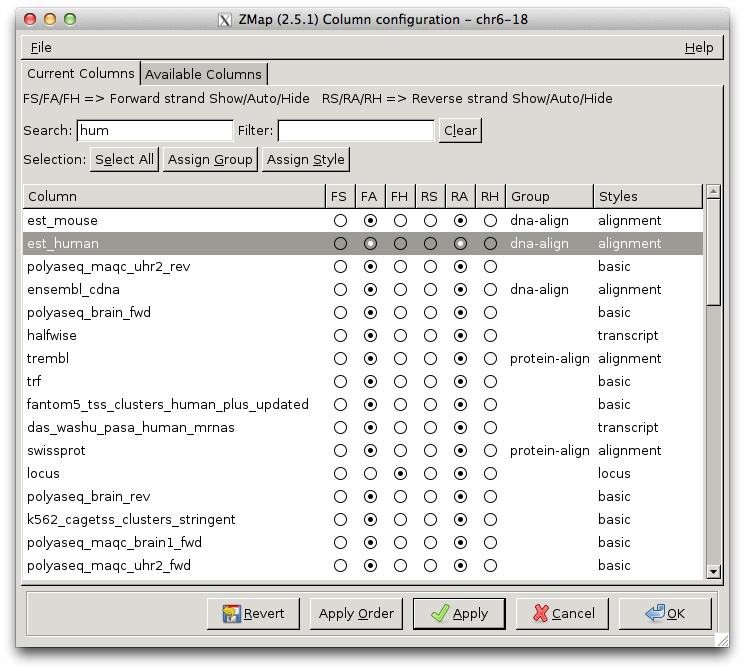
\includegraphics[width=15.231cm]{img_columns.png}
\caption{Columns dialog}
\label{img_columns}
\end{figure}


\subsection{Toolbar}
Many functions are available from the toolbar section in ZMap. See figures \ref{img_toolbar_feature_details} and \ref{img_feature_display_details}.

\begin{figure}
\centering
\color[rgb]{0.30980393,0.5058824,0.7411765}
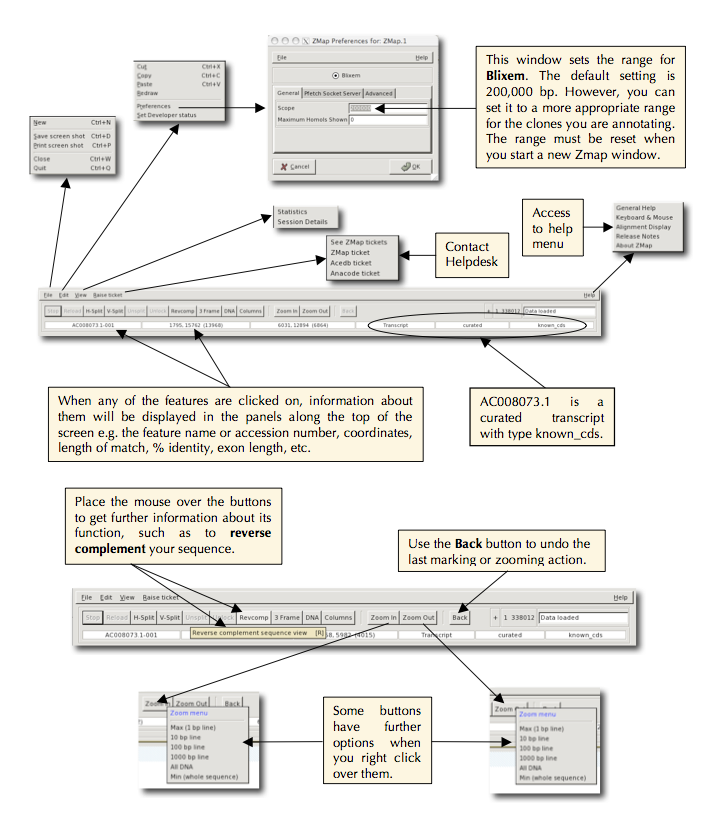
\includegraphics[width=15.231cm]{img_toolbar_feature_details.png}
\caption{Toolbar feature details}
\label{img_toolbar_feature_details}
\end{figure}

\begin{figure}
\centering
\color[rgb]{0.30980393,0.5058824,0.7411765}
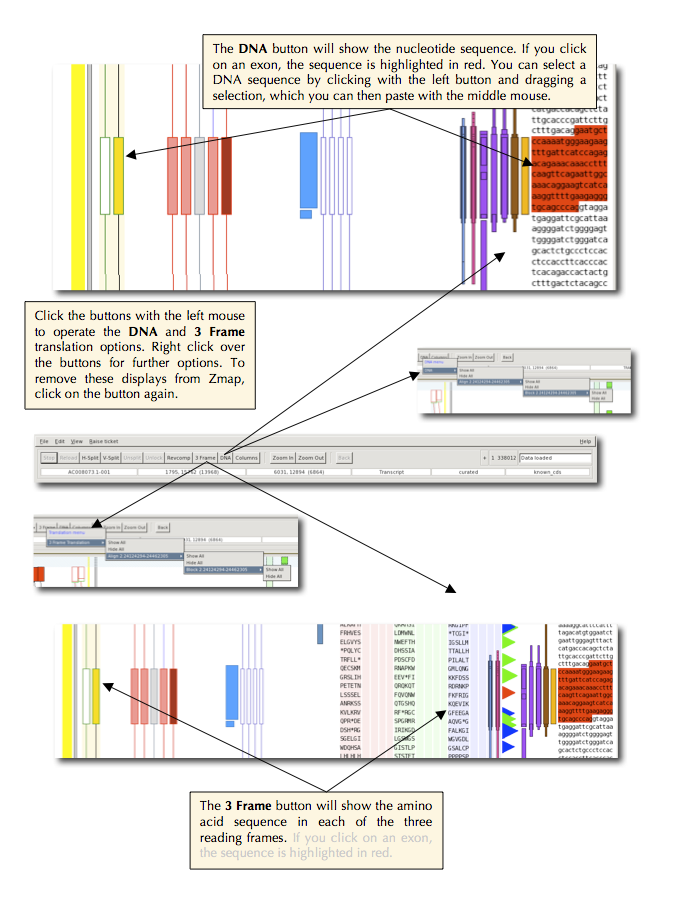
\includegraphics[width=15.231cm]{img_feature_display_details.png}
\caption{Feature display details}
\label{img_feature_display_details}
\end{figure}


\subsection{Show feature details}
Right click on a gene object or 'o' key when highlighted to see information on otter IDs and Ensembl IDs. For BLAST hits, double click on the HSP to get the feature interface where you will find details on alignment and on what gene object the HSP has been assigned to as evidence, if any (see figure \ref{img_feature_details_dialog}).

\begin{figure}
\centering
\color[rgb]{0.30980393,0.5058824,0.7411765}
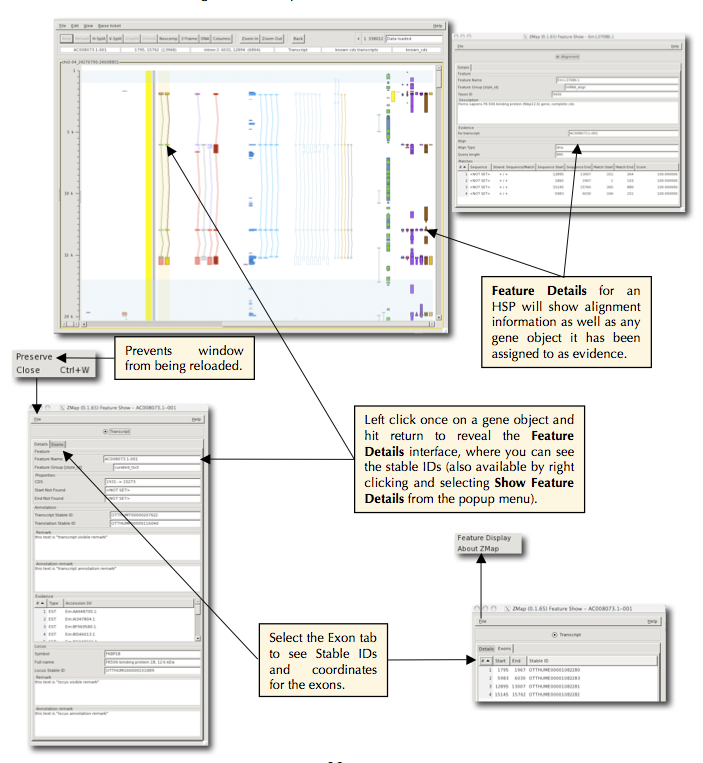
\includegraphics[width=15.231cm]{img_feature_details_dialog.png}
\caption{Feature details dialog}
\label{img_feature_details_dialog}
\end{figure}

\subsection{Exporting features for gene objects}
Figure \ref{img_exporting_features} shows how you can view and export an annotated sequence to your home directory in various different ways, such as dumping features directly.
\begin{enumerate}
\item In the main ZMap window, right click on an annotated gene object.
\item From the drop down menu select \textbf{Export Feature DNA} and choose sequence required from CDS, transcript, unspliced and with flanking sequence.
\item Alternatively, select \textbf{Export Feature peptide} and choose either CDS or transcript.
\item Figure \ref{img_exporting_features} also shows the results of \textbf{Show Feature DNA} for annotated gene object AC008073.1-001 in FASTA format; firstly, the section of the transcript that corresponds to the CDS and secondly the whole transcript, including the untranslated region (UTR).
\end{enumerate}

\begin{figure}
\centering
\color[rgb]{0.30980393,0.5058824,0.7411765}
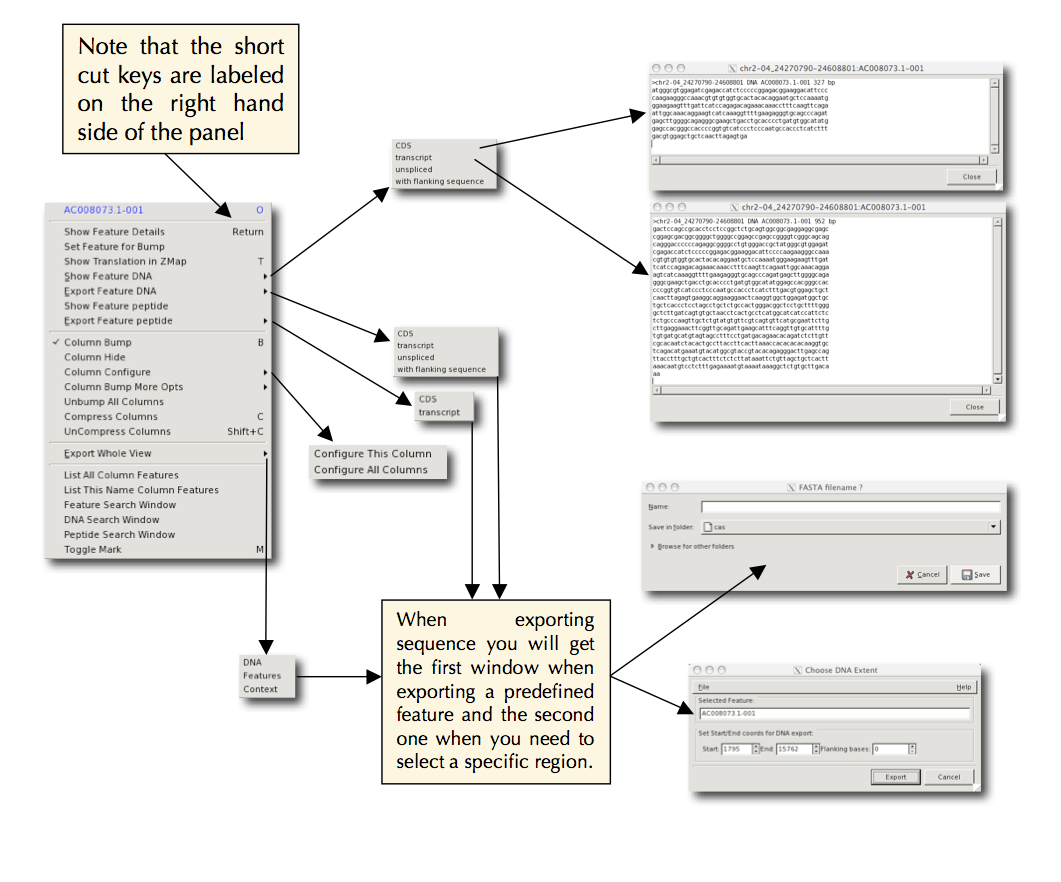
\includegraphics[width=15.231cm]{img_exporting_features.png}
\caption{Exporting features}
\label{img_exporting_features}
\end{figure}


\subsection{Bumping features}
This section describes how to select a feature, mark it and then zoom in to it and examine evidence that overlaps that feature. The default setting for ZMap is to show HSPs drawn on top of each other. This saves space on the canvas making it easier to see the general features of the region of interest. The bump option allows you to see the HSPs as multiple alignments.
\begin{enumerate}
\item Click on the feature you are interested in (perhaps a transcript)
\item Mark it by pressing "m"
\item Zoom in to the feature by pressing either "z" or "Z" (as described previously).
\end{enumerate}

\begin{figure}
\centering
\color[rgb]{0.30980393,0.5058824,0.7411765}
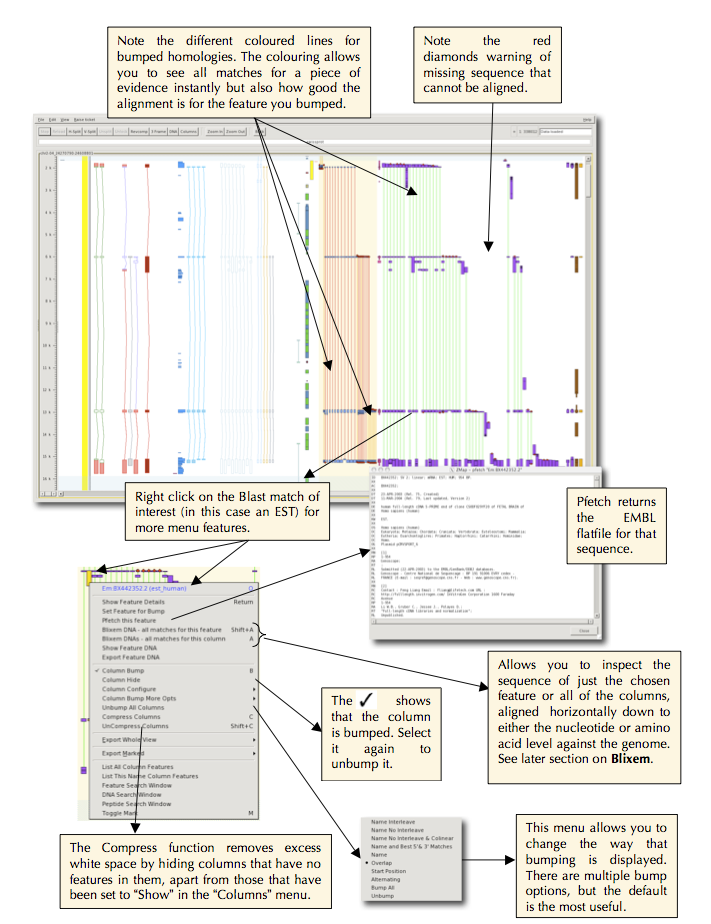
\includegraphics[width=15.231cm]{img_bumping.png}
\caption{Bumping features}
\label{img_bumping}
\end{figure}

Now when you bump an evidence column to look at matches that overlap the feature you will find that bumping is much faster because only those matches that overlap the feature get bumped and you also have fewer matches to look at. The quickest way to bump a column is:
\begin{enumerate}
\item Click on the column to select it.
\item Bump it by pressing "b" (if you press "b" again the column will be unbumped). If you have marked a feature then bumping is restricted to matches that overlap that feature, otherwise bumping is for the whole column.
\end{enumerate}

If you use the default bumping mode (i.e. you pressed "b") then you will find all matches from the same piece of evidence are joined by coloured bars, the colours indicate the level of colinearity between the matches (see figure \ref{img_bumping}).
\begin{enumerate}
\item \textcolor{darkgreen}{\textbf{Green}}: the matches at either end are perfectly contiguous, e.g. 100, 230 ---> 231, 351
\item \textcolor{orange}{\textbf{Orange}}:the matches at either end are colinear but not perfect , e.g. 100, 230 ---> 297, 351. Matches may also be this color when there are extra bases in the alignment, e.g. around clone boundaries.
\item \textcolor{red}{\textbf{Red}}: the matches are not colinear, e.g. 100, 230 ---> 141, 423
\end{enumerate}

Alignment quality of the HSPs is depicted by the width of every alignment displayed since the width is a measure of that HSP's score. Therefore, the wider it is the closer the score is to 100\%. The precise score is displayed in the ZMap details bar by clicking on the alignment. If HSPs are missing either the first or last Blast alignments in the set, they are marked with a red diamond at their start/end respectively. This indicates if they do not start at the first base/amino acid and/or do not end with the last base/amino acid of the alignment sequence. The screen shot below shows what options you get when you right click over a homology - note that you can also select an HSP and type ``o''. You also get further options such as retrieving the EMBL file for that homology using pfetch and starting \textbf{Blixem}, see later section (note, HSPs do not need to be bumped to use Blixem).

\subsection{Searching for a sequence in ZMap}
DNA and peptide search windows are provided from within ZMap and can be accessed by right clicking on ZMap space and selecting the option at the bottom of the menu. Both search windows are shown in figure \ref{img_sequence_search}.

\begin{figure}
\centering
\color[rgb]{0.30980393,0.5058824,0.7411765}
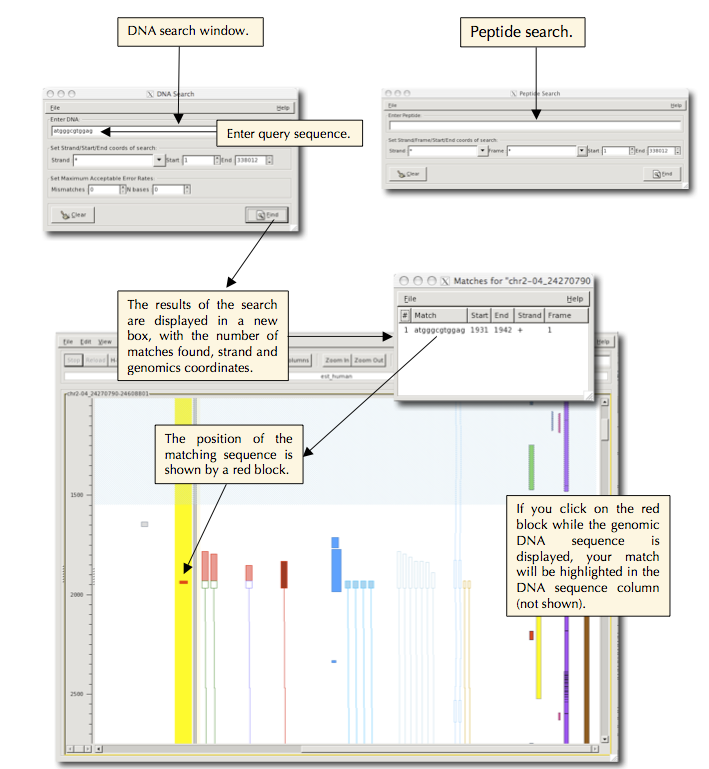
\includegraphics[width=15.231cm]{img_sequence_search.png}
\caption{Searching for a sequence}
\label{img_sequence_search}
\end{figure}

\subsection{Searching for a feature in ZMap}
This option allows you to list all the features contained in a column in one window. There are further options for you to search within these results to find a specific feature. The list of column features can be exported as a GFF file via the File menu. See figures \ref{img_feature_search} amd \ref{img_feature_search_results}.

\begin{figure}
\centering
\color[rgb]{0.30980393,0.5058824,0.7411765}
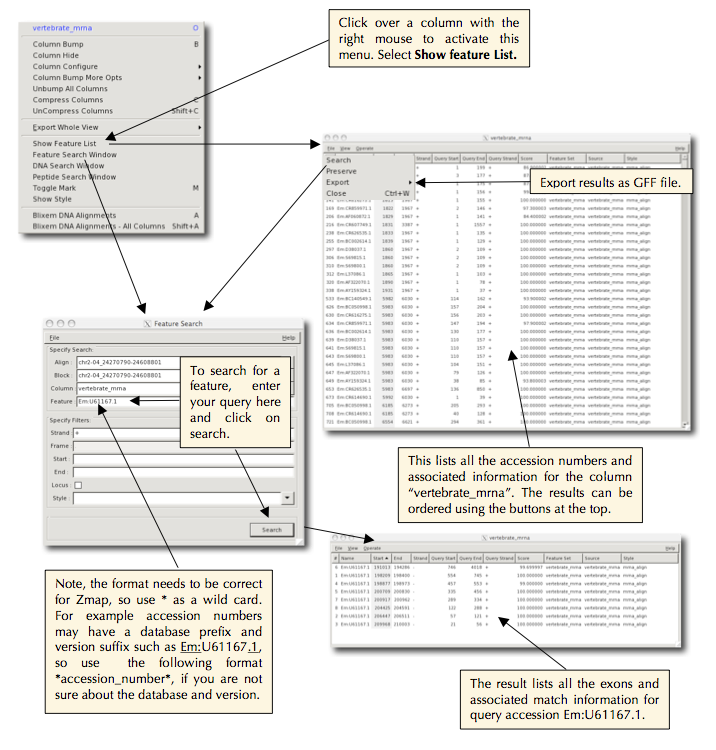
\includegraphics[width=15.231cm]{img_feature_search.png}
\caption{Searching for a feature}
\label{img_feature_search}
\end{figure}

\begin{figure}
\centering
\color[rgb]{0.30980393,0.5058824,0.7411765}
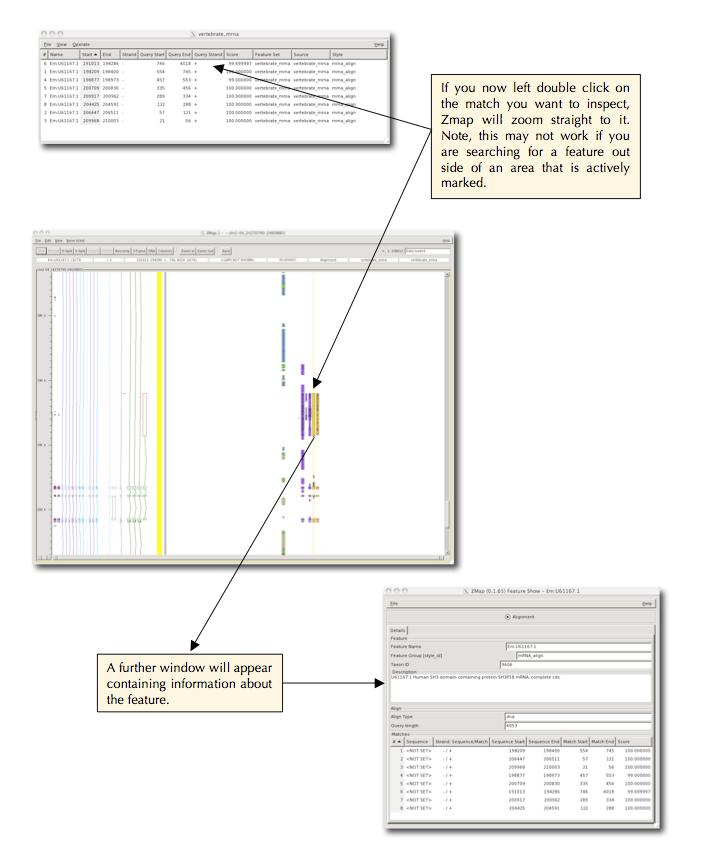
\includegraphics[width=15.231cm]{img_feature_search_results.png}
\caption{Feature search results}
\label{img_feature_search_results}
\end{figure}

\subsection{Selecting single or multiple features and hiding/showing them}
\begin{enumerate}
\item If you left click once on a feature in ZMap, you will highlight all of its exons, the coordinates of which are now stored in the paste buffer and can be copied elsewhere, such as into the transcript editing window in Otter.
\item You can select multiple features by holding the Shift key down and left clicking with mouse (same as for multi select on the Mac, Windows etc). This option will highlight a single exon at a time for each feature, but the accession numbers of each feature and the individual exon coordinates are held in the paste buffer. This is a particularly useful way of selecting ZMap hits to use in the OTF alignment tool in Otter, as all selected homologies will be held in the paste buffer and automatically pasted into the OTF accession window. Each of the exon coordinates can also be pasted into the transcript editing window in Otter (see figure \ref{img_show_hide}).
\item You can remove selected features in ZMap by pressing \textbf{Delete} on the keyboard and restore them by pressing \textbf{Shift-Delete} (note on the Mac you need to press \textbf{Fn-Delete} and \textbf{Shift-Fn-Delete}). This is a particularly useful way of removing evidence that you have already assigned to a transcript object.
\end{enumerate}


\begin{figure}
\centering
\color[rgb]{0.30980393,0.5058824,0.7411765}
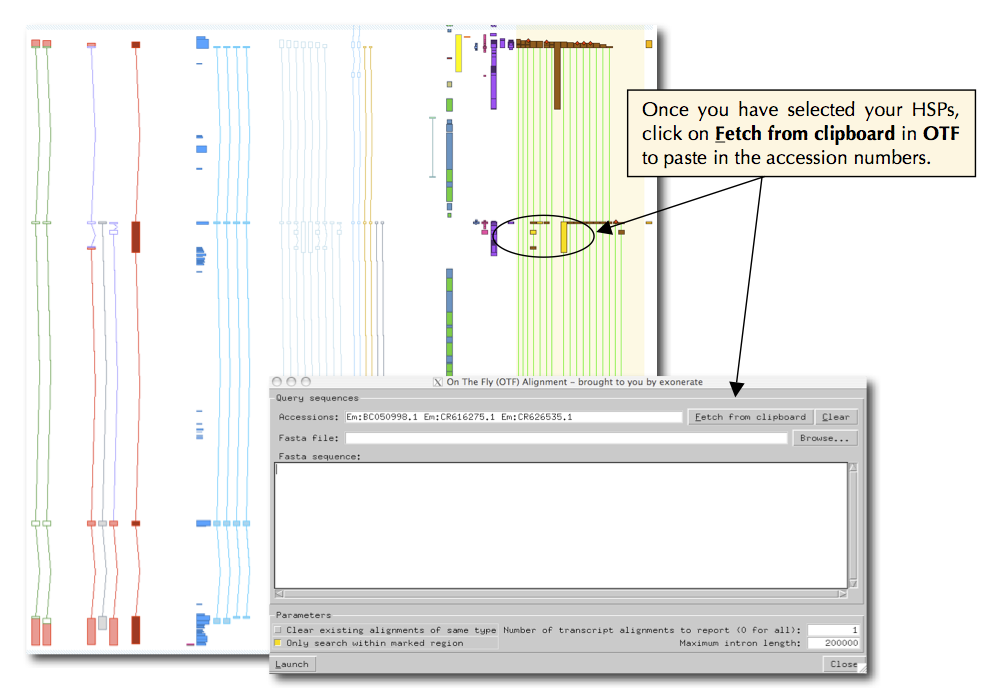
\includegraphics[width=15.231cm]{img_show_hide.png}
\caption{Pasting selected features to Otter's OTF dialog}
\label{img_show_hide}
\end{figure}


\subsection{Creating/editing features}
ZMap can be used to create new features or edit existing features. ZMap can generate variant objects quickly - existing transcript objects can be used as a template for a new object while a ZMap HSP (or any other feature, nucleotide or peptide) can be used to provide the coordinates for the new variant.

\subsubsection{Standalone ZMap}
Features are edited by copying them to a temporary feature in the \textbf{Annotation} column (see figure \ref{img_editing_zmap}). The Annotation functionality must first be enabled by ticking the \textbf{Enable Annotation} option in the preferences dialog. The temporary feature can be based on any existing feature(s). Multiple features or nucleotide coords can be used to adjust feature/exon coordinates. The coordinates and other attributes can also be edited manually. When finished, the temporary feature can be saved to the relevant column - either as a new feature, or to overwrite an existing one. 

The workflow is roughly as follows:
\begin{itemize}
\item Go to the menu option \texttt{Edit -> Preferences} and tick \texttt{Enable Annotation}
\item Right-click a feature and select \texttt{Annotation -> Copy this feature} to create the temporary feature
\item Copy other features/coordinates in the same manner to edit the temporary feature
\item Double-click the temporary feature to set a name/featureset and save it to that featureset
\item Right-click the new feature and select \texttt{Export -> Feature} to save the new feature to file
\end{itemize}

To create a new temporary feature, select the transcript (or other feature) you wish to create a variant from and press \textbf{Ctrl-K} (or right-click and select Annotation -> Copy selected transcript(s)\footnote{Note that you need to enable the Annotation column from the Preferences dialog for the Annotation menu to appear. Ctrl-K will automatically enable the Annotation column if it is not already enabled.}). Select other features and use Ctrl-K to copy those in to adjust the coordinates of the original feature. ZMap will do its best to make a sensible merge of the new coordinates, e.g. extending the feature extents if a coordinate lies outside the current range. If ZMap cannot automatically merge a coordinate it will ask for more information, e.g. if a coordinate lies within an intron, ZMap will ask whether it should form a 5' or 3' intron boundary.

The Annotation menu in the right-click menu also offers other options such as: clear the Annotation column; delete an exon/intron; undo/redo the last operation.

You can right-click the temporary feature and select \textbf{Highlight evidence} to highlight the feature(s) that were used to construct it.

\textbf{Double-click} the temporary feature to open the \textbf{Edit Feature} dialog to edit coordinates and other attributes manually. You can specify the new feature's final name and feature set. If you wish to save these attributes to the temporary feature (without saving the feature to the feature set) then click \textbf{Save Attributes}. To go ahead and save the feature to the named feature set, click \textbf{Create Feature}. You can overwrite an existing feature by giving the new feature the same name and featureset as the existing one. Note that to save the feature back to file you also need to \textbf{Save/Export} the relevant feature(s) by going to the File menu and selecting one of the Save or Export menu options.

\begin{figure}
\centering
\color[rgb]{0.30980393,0.5058824,0.7411765}
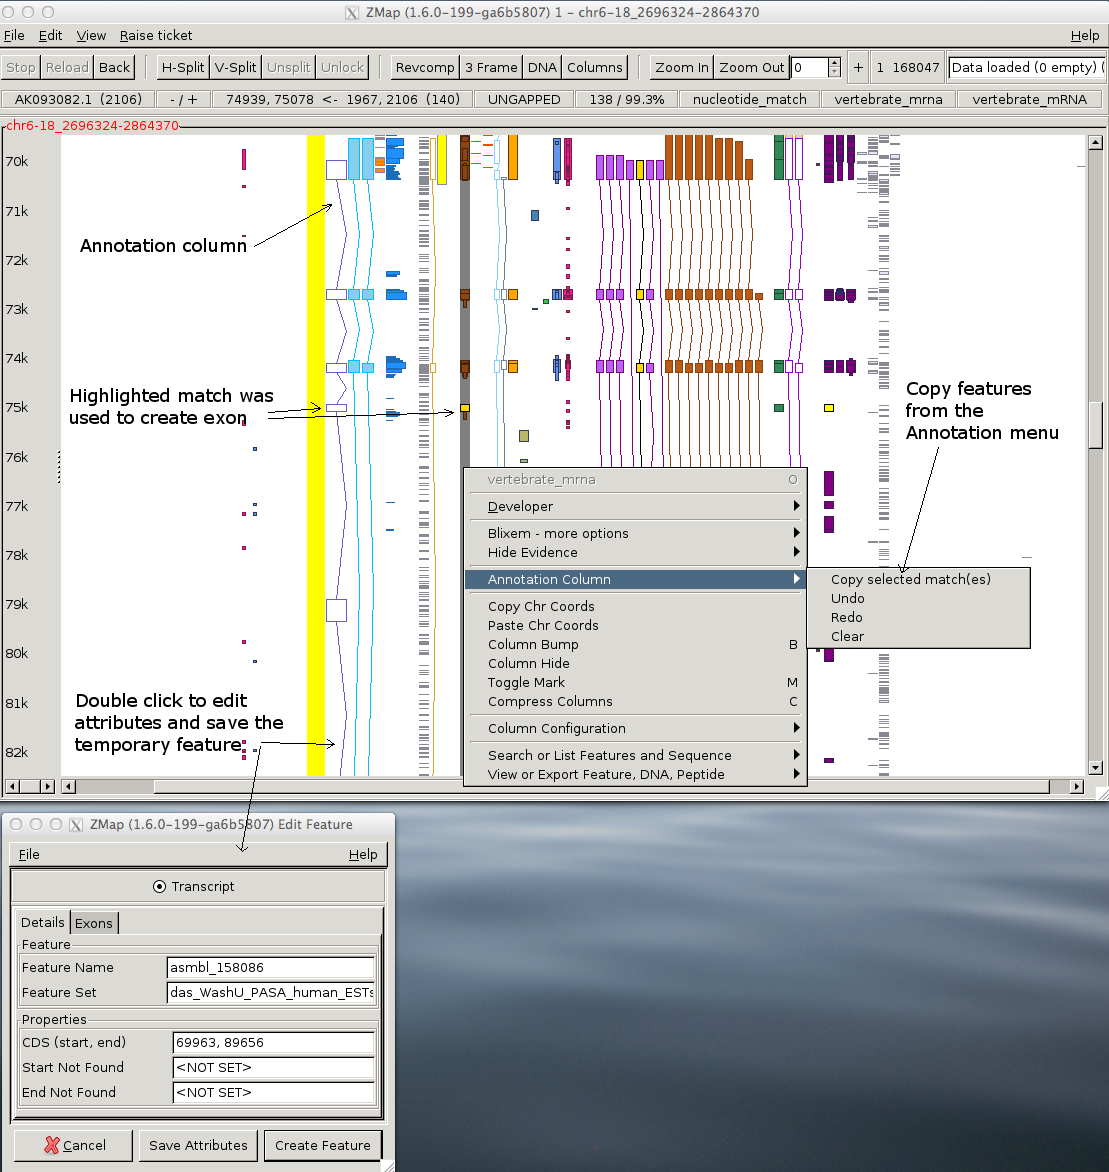
\includegraphics[width=15.231cm]{img_editing_zmap.png}
\caption{Feature editing in ZMap}
\label{img_editing_zmap}
\end{figure}

\subsubsection{Variant construction with Otter}
When running ZMap under Otter, variants are constructed in a different manner. See figures \ref{img_variant_construction} and \ref{img_variant_construction2}.

\begin{figure}
\centering
\color[rgb]{0.30980393,0.5058824,0.7411765}
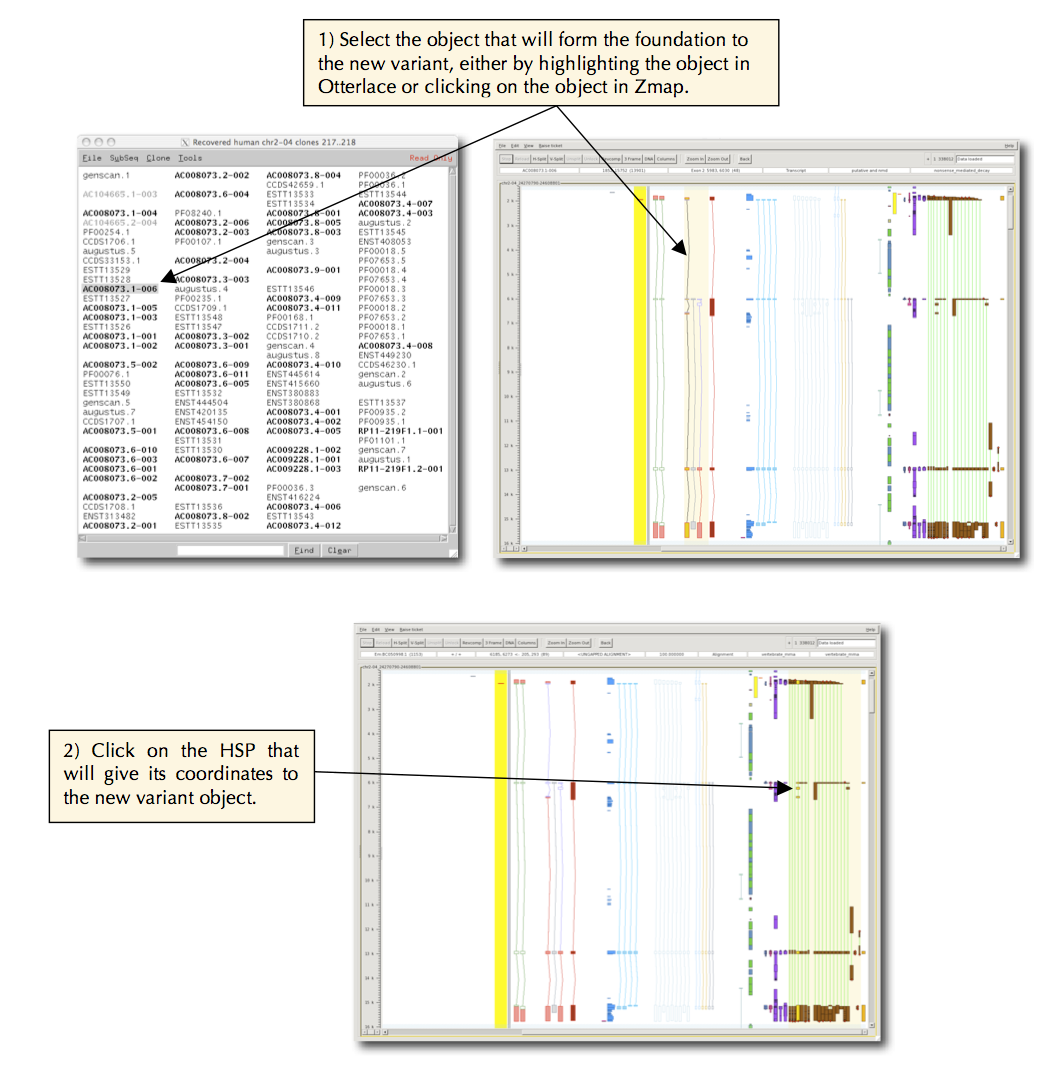
\includegraphics[width=15.231cm]{img_variant_construction.png}
\caption{Variant construction in Otter (1)}
\label{img_variant_construction}
\end{figure}

\begin{figure}
\centering
\color[rgb]{0.30980393,0.5058824,0.7411765}
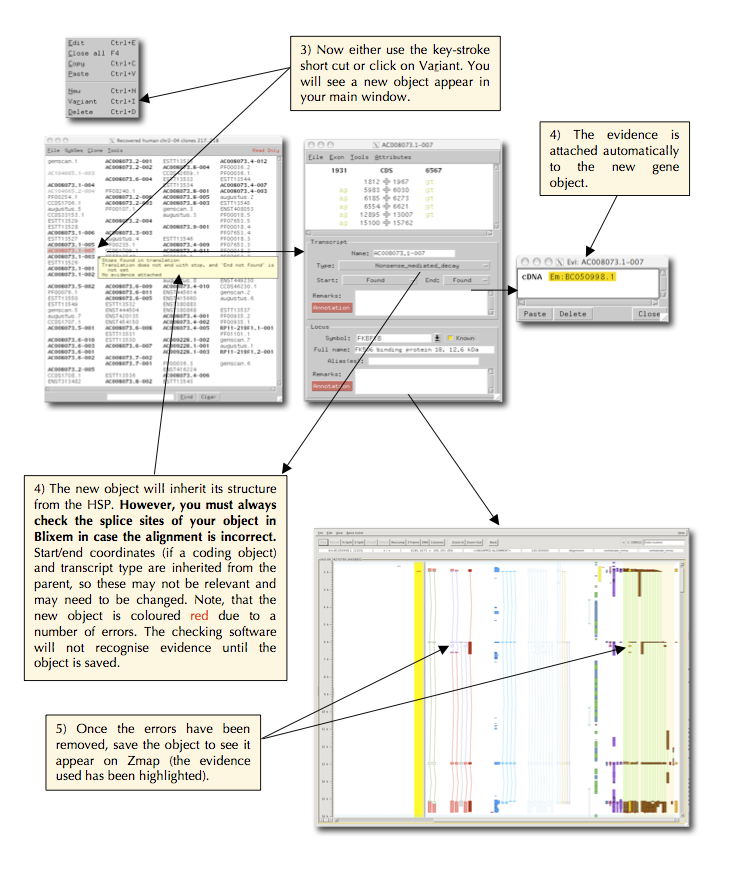
\includegraphics[width=15.231cm]{img_variant_construction2.png}
\caption{Variant construction in Otter (2)}
\label{img_variant_construction2}
\end{figure}

\subsection{Splitting windows in ZMap}
Use the \textbf{split} window function to effectively reduce the size of the window when looking at homologies. This is of particular use when you have to deal with very large introns because you can essentially reduce the introns to whatever size you wish, or when there are very many HSPs, because you can keep your gene object in view and static, but still scroll across the evidence. See figure \ref{img_split_window}.

\begin{figure}
\centering
\color[rgb]{0.30980393,0.5058824,0.7411765}
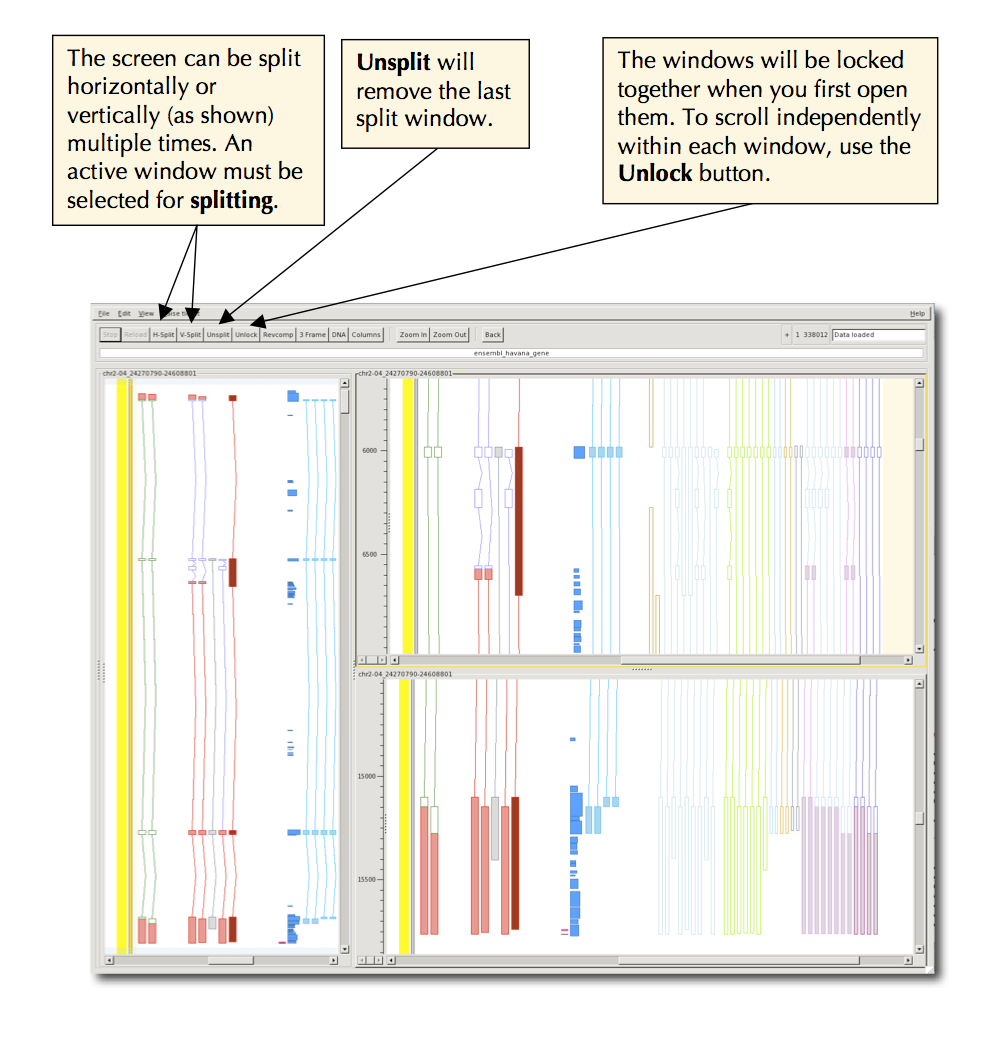
\includegraphics[width=15.231cm]{img_split_window.png}
\caption{Splitting windows}
\label{img_split_window}
\end{figure}

\subsection{Launching in a ZMap from Otter}
This function allows you to open two or more sequences alongside each other (such as a human region and the syntenic region in mouse, or two haplotypes), so that simultaneous investigation can be carried out. To do this you will need to open both sets of clones in the same Otter session. To open both ZMap windows in one window as shown below, you need to select "Launch In A ZMap" option in one clone set. These clones will open to the left of the already open Otter session. This screen shot shows human gene SF3B14 and the syntenic region in mouse. The gene copy and paste function (referred to in the Otter section) is of much use here, saving time when building gene objects. See figure \ref{img_launch_in_zmap}.

\begin{figure}
\centering
\color[rgb]{0.30980393,0.5058824,0.7411765}
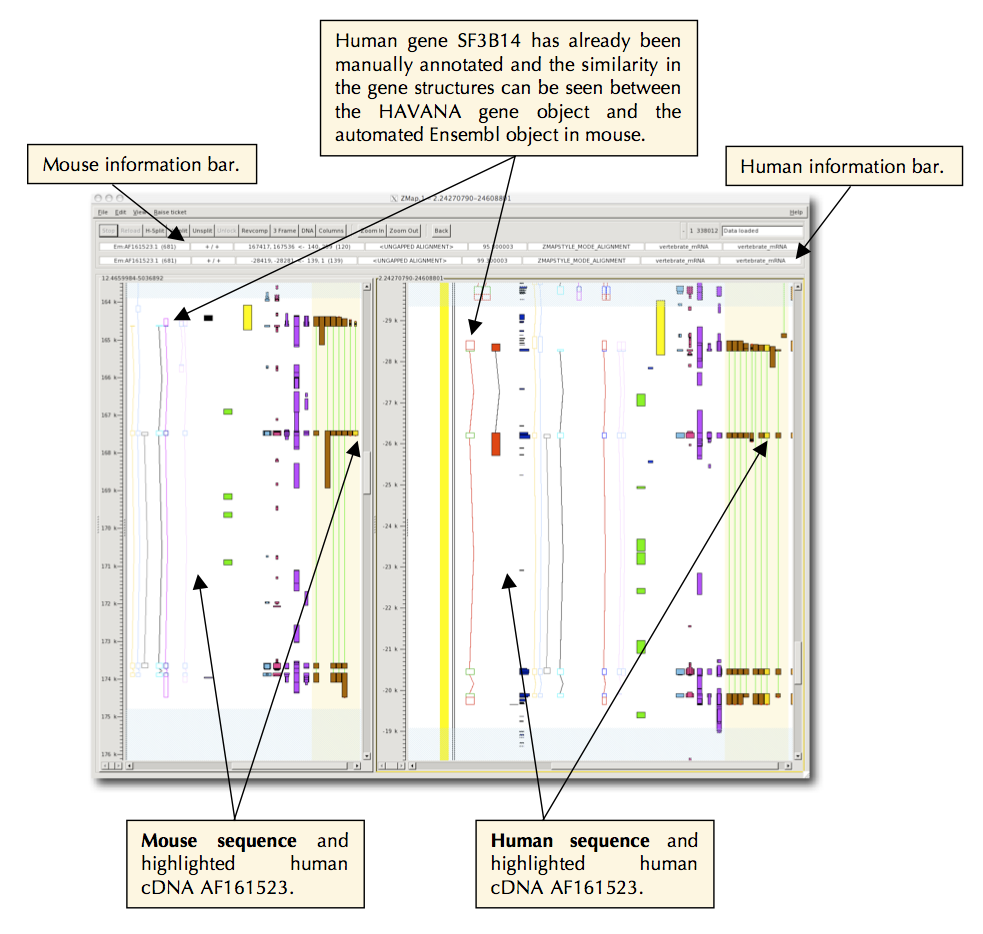
\includegraphics[width=15.231cm]{img_launch_in_zmap.png}
\caption{Launch in an existing ZMap}
\label{img_launch_in_zmap}
\end{figure}

\section{Keyboard and mouse shortcuts}
In general ZMap will be faster for zooming, bumping etc if you make good use of the built in short cuts. These can often avoid the need for ZMap to redraw large amounts of data that you may not even be interested in. For example, click once (highlight) on a feature and a carriage return will bring up evidence. Another example is to press T for translation.

\subsection{All windows}

\begin{supertabular}{|m{6cm}|m{8.5cm}|}
\hline
Short Cut & Action \\
\hline
Cntl-W & close this window \\
Cntl-Q & quit ZMap \\
\hline
\end{supertabular}

\subsection{ZMap Window}

\begin{supertabular}{|m{6cm}|m{8.5cm}|}
\hline
Short Cut & Action\\
\hline
\multicolumn{2}{|l|}{Control keys} \\
\hline
+ (or =), - & zoom in/out by 10\%\\
Cntl + (or =), Cntl - & zoom in/out by 50\%\\
up-arrow, down-arrow & scroll up/down slowly bit\\
Cntl up-arrow, Cntl down-arrow & scroll up/down more quickly\\
left-arrow, right-arrow & scroll left/right slowly\\
Cntl left-arrow, Cntl right-arrow & scroll left/right more quickly\\
page-up, page-down (Mac users should use fn and up/down arrow) & up/down by half a "page"\\
Cntl page-up, Cntl page-down & up/down by a whole "page"\\
Home, End (Mac users should use fn and left/rights arrows) & Go to far left or right\\
Cntl Home, Cntl End (Mac users will have to configure their keyboards for this) & Go to top or bottom\\
Delete, Shift Delete & Hide/Show selected features.\\
Enter & Show feature details for highlighted feature.\\
Shift up-arrow, Shift down-arrow & Jump from feature to feature within a column.\\
Shift left-arrow, Shift right-arrow & Jump from column to column.\\
Cntl-K & Copy selected feature(s) to the Annotation column for editing. Also enables Annotation if not already enabled.\\
\hline
\end{supertabular}

\subsection{Alpha-numeric keys}
\begin{supertabular}{|m{1.5cm}|m{13cm}|}
\hline
Short Cut & Action\\\hline
a & Blixem all sequences in column\\
A & Blixem only highlighted sequence in column\\
b & Bump/unbump current column within limits of mark if set, otherwise bump the whole column.\\
B & Bump/unBump current column within limits of the visible feature range.\\
c & compress/uncompress columns: hides columns that have no features in them either within the marked region or if there is no marked region within the range displayed on screen. Note that columns set to "Show" will not be hidden.\\
C & Compress/unCompress columns: hides all columns that have no features in them within the range displayed on screen regardless of any column, zoom, mark etc. settings.\\
h & Toggles highlighting (good for screen shots).\\
m & mark/unmark a range which spans whichever features or subparts of features are currently selected for zooming/smart bumping\\
M & Mark/unMark the whole feature corresponding to the currently selected subpart (e.g. the whole transcript of an exon or all HSPs of the same sequence as the highlighted one) for zooming/smart bumping\\
o or O & show menu Options for highlighted feature or column, use cursor keys to move through menu, press ESC to cancel menu.\\
r & reverse complement current view, complement is done for all windows of current view.\\
t or T & translate highlighted item, T hides Translation.\\
w or W & zoom out to show whole sequence\\
z & zoom to the extent of any selected features (e.g. exon/introns, HSPs etc) or any rubberbanded area if there was one.\\
Z & Zoom to whole transcript or all HSPs of a selected feature.\\
\hline
\end{supertabular}

\subsection{ZMap Mouse Usage}
\begin{supertabular}{|m{4.8cm}|m{4.8cm}|m{4.8cm}|}
\hline
Left & Middle & Right\\
\hline
\textit{Single mouse button click} & & \\\hline
highlight a feature or column
Plus drag: draw a rectangle around an object for zoom &
horizontal ruler with sequence position displayed, on button release centre on mouse position.
Release mouse outside ZMap window to prevent re-centering.&
show feature or column menu - for options such as pfetch, show feature DNA, show peptide, export peptide\\
\hline
\textit{Double mouse button click} & & \\\hline
display details of selected feature. Double click on object to get edit window&
same as single click&
same as single click\\
\hline
\textit{Shift + mouse button click} & & \\\hline
highlight a subpart of a feature (e.g. a single exon or alignment match)
OR multiple highlight&
same as single click&
same as single click\\
\hline
\end{supertabular}

\section{Tips for a speedier ZMap}
\begin{enumerate}
\item Specifically: zoom and mark within ZMap early on after launching. Either select a gene object and press 'z' to zoom OR select a rectangle to zoom in by dragging the left mouse button around it. Reverse complement now if necessary, then press 'm' to mark the region.
\item The quickest way to zoom out of ZMap again is to right mouse click on the 'zoom out' buttons at the top of zmap and choose one of the options (this is definitely much quicker that doing individual 'zoom outs' with the left mouse button). Likewise for 'zooming in' again (or use keyboard equivalents).
\item Bump within a marked region only. Bumping without marking is slow and removes the lines connecting Blast matches.
\item When you have finished working within a marked region, unbump the evidence you have been working on (e.g. ESTs) and unmark that region before you go on to select the next region to mark and bump - or you could miss visualising the evidence in the new region.
\item If you want to get rid of some white space try the compress 'c' function or alternatively toggle off some of the columns. \textcolor{red}{Warning - this may hide features as well}. If a column (e.g ESTs) is bumped and you want to lose it temporarily, it is quicker to turn the column off (when you turn it on again it will still be bumped when it re-appears) than unbump then rebump again later.
\item Jumping to genes/objects: If you expand the left hand 'scroll navigator' overview' you can jump directly to genes and objects by double-clicking on them.
\end{enumerate}

\end{document}
